\subsection{BERT}

BERT — Bidirectional Encoder Representations from Transformers (Двунаправленные кодировочные представления на основе трансформеров). В отличие от других моделей языкового представления (Peters, Radford и др), BERT разработан для предварительного обучения глубоких двунаправленных представлений на неразмеченном тексте, при этом модель одновременно учитывает как левый, так и правый контекст на всех слоях.

В результате, предварительно обученную модель BERT можно дообучить (fine-tune), добавив всего один выходной слой, чтобы получить модели состояния искусства (state-of-the-art) для широкого спектра задач, таких как ответы на вопросы и логический вывод из текста, без необходимости в значительных модификациях архитектуры под конкретную задачу.

С концептуальной точки зрения BERT — простая, но с эмпирической точки зрения — мощная модель. Она показывает высокие результаты в NLU тестах  на одиннадцати задачах обработки естественного языка, включая:
\begin{itemize}
   \item увеличение общего балла GLUE до 80.5\%,
   \item увеличение точности на MultiNLI до 86.7\%,
   \item увеличение F1-метрики на тесте SQuAD v1.1 до 93.2 (улучшение на 1.5\%) и F1-метрики на тесте SQuAD v2.0 до 83.\1% /

\end{itemize}


Архитектура модели BERT представляет собой многослойный двунаправленный кодировщик на основе трансформеров и выпущенной в библиотеке tensor2tensor.

Чтобы адаптировать BERT к разнообразным прикладным задачам, модель ввода была разработана так, чтобы однозначно представлять как одно предложение, так и пару предложений (например, вопрос и ответ) в одной последовательности токенов.

В рамках данной работы под «предложением» понимается произвольный фрагмент связанного текста, а не обязательно грамматически завершённое предложение. «Последовательность» обозначает входную последовательность токенов для BERT, которая может содержать как одно предложение, так и два объединённых.

Для представления токенов используются эмбединги WordPiece  с словарём из 30000 токенов. Первый токен любой последовательности — это специальный классификационный токен [CLS]. Его последнее скрытое состояние используется как суммарное представление всей последовательности при решении задач классификации.

Пары предложений объединяются в одну последовательность. Для их различения применяются два механизма:


\begin{enumerate}[label=\arabic*.]
\item Между предложениями вставляется специальный токен [SEP];

\item К каждому токену добавляется обучаемый эмбединг, указывающий, принадлежит ли он предложению A или B.
\end{enumerate}

Как показано на рисунке 2, входной эмбеддинг обозначается как \( E \), финальный скрытый вектор токена \([CLS]\) — как \( C \in \mathbb{R}^H \), а финальный скрытый вектор для \( i \)-го токена — как \( T_i \in \mathbb{R}^H \).

\begin{figure}[h!]
    \centering
    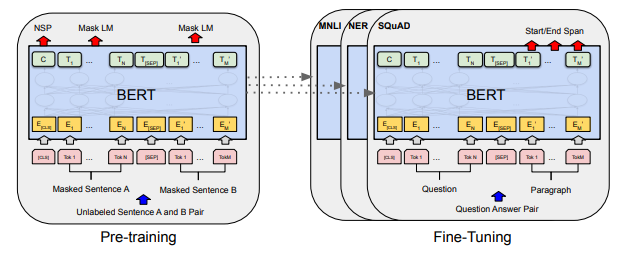
\includegraphics[width=0.7\textwidth]{styles/diploma/inc/bert1.png} 
    \caption{Общая схема предварительного обучения и дообучения модели BERT

}
    \label{fig:example}
\end{figure}


Для любого токена его входное представление формируется путём суммирования трёх компонентов:
\begin{enumerate}[label=\arabic*.]
\item эмбединга токена,

\item эмбединга сегмента (указывающего, к какому предложению он относится),
\item позиционного эмбединга.
\end{enumerate}


Визуализация этого процесса представлена на рисунке 3.

   \begin{figure}[h!]
    \centering
    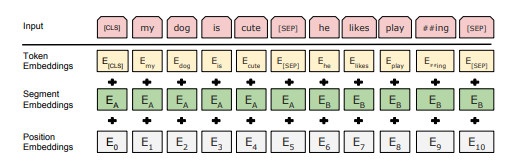
\includegraphics[width=0.7\textwidth]{styles/diploma/inc/bert2.png} 
    \caption{Представление входных данных в BERT}
    \label{fig:example}
\end{figure}

BERT не использует традиционные языковые модели, обучаемые слева направо или справа налево, для предварительного обучения BERT. Вместо этого модель обучается  на основе двух задач без учителя, описанных в этом разделе. Этот этап изображён в левой части рисунка 2

нтуитивно понятно, что глубокая двунаправленная модель потенциально более мощная, чем слева-направо модель или неглубокая конкатенация двух однонаправленных моделей. Однако стандартные условные языковые модели могут обучаться только в одном направлении, поскольку двунаправленная модель позволила бы каждому слову "видеть само себя", что делало бы предсказание тривиальным.

Чтобы обучить действительно двунаправленное представление, случайный процент токенов  маскируется во входной последовательности, и модель обучаеется  предсказывать эти токены. Эта  процедура называется  Masked Language Model (MLM) (в литературе также известна как Cloze-задача). Векторы, соответствующие маскированным токенам, подаются на выходной слой softmax поверх словаря, аналогично стандартной языковой модели.

Во всех наших экспериментах  случайным образом маскируются 15\% токенов WordPiece в каждой последовательности.

В отличие от автокодировщиков с устранением шума, здесь  предсказываются только замаскированные токены, а не восстанавливается вся последовательность.

Проблема в том, что токен [MASK] не встречается во время дообучения, что создаёт рассогласование между этапами обучения и применения. Чтобы сгладить это расхождение, выбранные токены  не всегда заменяются на [MASK]. Генератор обучающих данных действует следующим образом:

\begin{enumerate}[label=\arabic*.]
\item выбирается 15\% позиций токенов для предсказания;

\item если выбран $i-й$ токен, он заменяется:
\begin{enumerate}[label=\arabic*.]
\item на [MASK] — в 80\% случаев;
\item на случайный токен — в 10\% случаев;
\item остаётся неизменным — в 10\% случаев.
\end{enumerate}

\end{enumerate}
Затем соответствующий скрытый вектор $T_i$ используется для предсказания исходного токена с использованием функции потерь кросс-энтропии.

Многие прикладные задачи, такие как вопросно-ответные системы (QA) и логический вывод (NLI), требуют понимания связей между двумя предложениями, чего не обеспечивает языковое моделирование.

Для этого мы обучаем модель на бинарной задаче предсказания следующего предложения (NSP), которую легко сгенерировать из любого одноязычного корпуса.

Для каждой обучающей пары предложений A и B:в 50\% случаев B действительно следует за A (метка IsNext),в 50\% случаев B — это случайное предложение из корпуса (метка NotNext).

Как показано на рисунке 2, для задачи NSP используется вектор [CLS], обозначаемый как C.

Несмотря на простоту, в разделе 5.1 показано, что предобучение на этой задаче существенно улучшает производительность как в QA, так и в NLI.

 BERT передаёт все параметры модели для инициализации downstream-задач.

Данные для предварительного обучения


Процедура предварительного обучения в целом соответствует предыдущим исследованиям по языковым моделям. Мы используем два корпуса:
\begin{enumerate}[label=\arabic*.]
\item BooksCorpus (~800 млн слов),

\item англоязычная Википедия (~2.5 млрд слов).
\end{enumerate}
Из Википедии извлекаются только текстовые блоки — списки, таблицы и заголовки игнорируются.

\subsubsection{Дообучение BERT(Fine-tuning)}


Дообучение BERT выполняется просто, так как механизм самовнимания (self-attention) в трансформере позволяет использовать модель для многих задач, включая как отдельные тексты, так и пары текстов, просто заменяя входы и выходы.

Обычно в задачах с парами текстов применяют двухэтапный подход: сначала кодируют предложения по отдельности, а затем применяют перекрёстное внимание (cross-attention), как в работах Parikh и др. (2016), Seo и др. (2017).

BERT же объединяет эти этапы — кодирует сразу объединённую пару предложений с помощью self-attention, тем самым реализуя перекрёстное внимание автоматически.

Для каждой задачи  подключаются специфичные входы и выходы, и модели дообучивают всеми параметрами  от начала до конца.

На входе:

пара предложений A и B, аналогичная: <добавить нормальтный спиолк>
\begin{enumerate}[label=\arabic*.]
\item парафразам;
\item паре гипотеза–предпосылка в задачах логического вывода;
\item паре вопрос–текст в QA;
\item паре «текст–∅» в классификации или теггинге последовательностей.
\end{enumerate}

На выходе:
\begin{enumerate}[label=\arabic*.]
\item вектор токена используется для задач на уровне токенов (sequence tagging, QA),
\item вектор [CLS] используется для задач классификации (например, sentiment analysis, entailment).
\end{enumerate}
паре гипотеза–предпосылка в задачах логического вывода;

паре вопрос–текст в QA;

паре «текст–∅» в классификации или теггинге последовательностей.

На выходе:

вектор токена используется для задач на уровне токенов (sequence tagging, QA),вектор [CLS] используется для задач классификации (например, sentiment analysis, entailment).

Итоги предварительного обучения BERT:

\begin{enumerate}[label=\arabic*.]
\item Характеристика	Подробности
Корпус для пре-тренинга	BookCorpus ≈ 800 млн слов + англ. Wikipedia ≈ 2,5 млрд слов (в сумме ≈ 3,3 млрд).
\item Модели	BERT-BASE (12 блоков, 768 скрытых, 12 голов, 110 M парам.).
\item BERT-LARGE (24 блока, 1024 скрытых, 16 голов, 340 M парам.) 
arXiv.
\item Задачи пре-тренинга	1. Masked LM (MLM) — случайно маскируются 15 \% токенов и предсказываются.
\itemКлючевые результаты	Новый SOTA на 11 NLP-бенчмарках: GLUE 80,5 (+7,7 pp), MultiNLI 86,7 (+4,6 pp), SQuAD v1.1 F1 93,2 (+1,5 pp) и др. 
arXiv.
\end{enumerate}

Результаты оригинального BERT впечатляют, но из-за английского корпуса они напрямую не переносятся на русский. Для качественной работы стоит сразу брать модель, предобученную на русском и, при необходимости, дообучать её на собственной задаче.

